\paragraph{Shared-feature retraining and revised execution.}
The version-2 router retains the $8\!\rightarrow\!32\!\rightarrow\!16$
network with one repair head and three scope outputs (884 parameters),
seed 42, and the original document-group split. Training fits the scaler
only on the 2,098 training rows; validation and test each contain 450 rows.
Repair classification and dominant-scope accuracy are 100\% on this
controlled test split. The repair Brier score is $1.02\times10^{-9}$.
These labels follow the known corruption construction; the result measures
recognition of those defects.

\begin{table}[t]
\centering
\caption{Version-2 selector on the same archived proposals. Relative priors use the uniform distribution as their zero point. Accepted edits are controlled / natural.}
\label{tab:math_revision_selector}
\small
\begin{tabular}{lrrr}
\toprule
Prior / offset & Controlled F1 & Natural F1 & Accepted \\
\midrule
Uniform / absolute & 0.8472 & 0.8833 & 0 / 10 \\
Uniform / relative & 0.8472 & 0.8833 & 0 / 10 \\
Learned / absolute & 0.8472 & 0.8799 & 0 / 10 \\
Learned / relative & 0.8929 & 0.8764 & 156 / 51 \\
\bottomrule
\end{tabular}
\end{table}


We execute four fixed router/utility combinations on the same 225 controlled
and 225 natural-input proposals (1,800 outcomes). Table~\ref{tab:math_revision_selector}
reports the revised implementation separately from the frozen component study
above. The revised uniform default evaluates 471 controlled candidate trials,
compared with 220 previously, but still accepts no edits. Candidate evaluation
alone therefore does not remove the positive-utility barrier.
With the retrained prior, the relative offset raises controlled F1 from
84.72\% to 89.29\%, while natural-input F1 changes from 87.99\% to 87.64\%.
The uniform alternatives give identical outputs. The default absolute offset
is retained; the contrast shows that a threshold shift can help one cohort
and harm another. The empty-value diagnostic fix changes no archived case.
All these proposals were previously evaluated, so this is a fixed-candidate
execution comparison. It does not alter the main one-call repair results.

\begin{figure}[t]
\centering
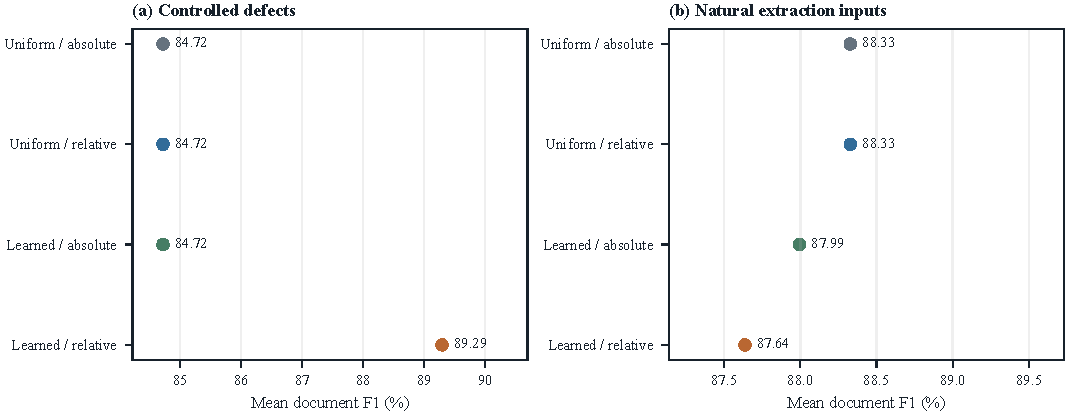
\includegraphics[width=0.98\textwidth]{figure/experiments/math_revision.pdf}
\caption{Revised selector with shared training and execution features. Points
show mean document F1 for fixed prior and offset choices on archived proposals.}
\label{fig:math_revision}
\end{figure}
